



\vfill

\stars

{\raggedleft
\textit{
Cet hiver a des airs de printemps\\
Des peuples ou de l'esprit, au diable l'âme.\\
Le vent se lève, ça faisait longtemps\\
Triste de s'enfermer pour quelques grammes.\\
}
}
\medskip

{\raggedright

\textit{
Cet avenir des airs de passé\\
S'il fallait juste trouver le régime,\\
Assassinée la complexité\\
Maintes perspectives se cachent en les crimes.\\
}
}

\medskip
{\raggedleft

\textit{
Pour une morphogenèse politique\\
Adieu le coron, ses tristes briques\\
Murs qui s'érigent tuent votre espérance.\\
}
}

\medskip
{\raggedright


\textit{
Perle de la mer, sirène hante la crique\\
Du haut des tours s'amuser du cirque\\
L'hiver d'idées qui peuple la France.\\
}
}

\stars

\vfill




%------------------------------------


\newpage






%\chapter*{Conclusion}{Conclusion}
\bpar{
\chapter*{Conclusion}
}{
\chapter*{Conclusion}
}



% to have header for non-numbered introduction
\markboth{Conclusion}{Conclusion}


\bpar{
\headercit{Keeping on exploring geographical systems\ldots}{Arnaud Banos}{}
}{
\headercit{Explorer sans relâche les systèmes géographiques\ldots}{Arnaud Banos}{}
}

% not appropriate (removed incipit)
% Le lecteur qui aura tenu jusqu'ici et qui a la mémoire solide ou bien sélective, ou encore qui aura adopté un style de lecture roman policier, se plaindra du manque d'originalité dans l'origine des citations introductives.


\bpar{
Our thesis is a complex system which exhibits an auxiliary deterministic finality: this conclusion by a citation of \noun{Banos}. Principles of its context, simple but efficient and deep, indeed flow through this work: the ``9 principles of Banos'' are implicitly present in most of the work done and of the perspectives opened. Even if an ideal application of these principles would be achieved by a ``Banos Deamon'', similar to the Laplace or Maxwell Deamon, which would be able to articulate interdisciplinary and disciplinary without being lost while respecting all the principles, their understanding as a scientific utopia, naturally reflexive and thus evolutive and adaptive, seems a powerful entry for new integrative approaches of territorial systems.
}{
Notre thèse est un système complexe qui exhibe une finalité auxiliaire déterministe : cette conclusion par un adage de \noun{Banos}. Les principes de son contexte, simples mais efficaces et profonds, traversent en effet ce travail : les ``9 principes de Banos'' sont implicitement présents dans la majorité des travaux menés et perspectives ouvertes. Même si une application idéale de ces principes relèverait d'un ``Démon de Banos'', à l'instar du Démon de Laplace ou de Maxwell, qui serait capable d'articuler interdisciplinaire et disciplinaire sans se perdre tout en respectant l'ensemble des principes, leur appréhension comme utopie scientifique, naturellement réflexive donc évolutive et adaptive, nous semble une entrée puissante pour de nouvelles approches intégratives des systèmes territoriaux. 
}


\bpar{
Our epistemological and methodological contribution in relation with these points is essential, even if it remains difficult to explicit and will necessitate a certain step back to be effectively understood. In a way, we brought an additional brick as a \emph{proof-of-concept} of the banosian system of principles, but also as an implementation and a deepening of it on some points. We have shown that their application is far from being simple, and that the risk of fall into reductionist is never far around the corner despite these fundamentally complex principles. The tenth commandment would it then be: \textit{aiming at applying these principles while always keeping in sight complexity and the role of reflexivity}?
}{
Notre contribution épistémologique, méthodologique en lien avec ces points est essentielle, même si celle ci est difficile à expliciter et nécessitera un certain recul pour être effectivement cernée. D'une certaine manière, nous avons apporté une brique supplémentaire comme \emph{proof-of-concept} du système de principes banosien, mais également comme implémentation et approfondissement de celui-ci sur certains points. Nous avons montré que leur application est loin d'être simple, et que toujours guette le risque de sombrer dans le réductionnisme malgré ces principes fondamentalement complexes. Le dixième commandement serait-il alors : \textit{S'efforcer à appliquer ces principes en ne perdant jamais de vue la complexité et le rôle de la réflexivité} ?
}


\bpar{
Our thematical contribution is not necessarily easy to situate and will necessitate a considerable step back to highlight its implications. Did we solve the gordian knot of co-evolution? Did we cut it? The most honest answer would be that we cut a part of it, the naive one including the definition from which we started in introduction or positioning of type ``chicken-and-egg'' typical of debates on structuring effects, but that we tied an other much more considerable, by unveiling the complexity of this concept and its manifestations.
}{
Notre contribution thématique n'est pas forcément facile à situer et nécessitera un recul considérable pour appréhender ses implications. Avons-nous résolu le noeud gordien de la co-évolution ? L'avons-nous tranché ? La réponse la plus fidèle serait que nous en avons tranché une partie, celle naïve comprenant la définition dont nous sommes parti en introduction ou les positionnement de type ``poule-et-oeuf'' typique des débats des effets structurants, mais que nous avons noué un autre bien plus considérable, en révélant la complexité de ce concept et de ses manifestations.
}


\bpar{
Coming back to our funding problematic, we recall that (i) we gave a definition of co-evolution proper to territorial systems and also an operational method of caracterization; (ii) we explored modeling directions at different scales, which articulate with a more global theoretical frame. Answer to this problematic furthermore allowed us to progressively build a broader frame and vast research perspectives.
}{
Revenant à notre problématique fondatrice, nous rappelons que (i) nous avons donné une définition de la co-évolution propre aux systèmes territoriaux ainsi qu'une méthode opérationnelle de caractérisation ; (ii) nous avons exploré des pistes de modélisation à différentes échelles, qui s'accordent avec un cadre théorique global. Répondre à cette problématique nous a permis par ailleurs de progressivement dégager un cadre plus large et de vastes perspectives de recherche.
}


\bpar{
Our modest mission is accomplished, and a fantastic journey only begins. The provisory accomplishment becomes the foundations of the ones to come. Cumulativity of knowledge is not improvised, and we suggest that the complex fabric of which we sew the first stitches will be robust enough to be inserted within. \textit{The road is long but the path is free.}
}{
Notre modeste mission est accomplie, et un fantastique voyage commence tout juste. L'accomplissement passager devient les fondations de ceux à venir. La cumulativité des connaissances ne s'improvise pas, et nous espérons que le tissu complexe dont nous avons cousu les premières mailles sera assez robuste pour s'y insérer. \textit{la route est longue mais la voie est libre.}
}




\stars










%%%%%%%%%%%%%%%%%%%%
%% Add epilogue -> may be separated




%\chapter{When Science meets Art}{Quand la science se mêle à l'art} % Chapter title

%\label{app:art} % For referencing the chapter elsewhere, use \autoref{ch:name} 

%----------------------------------------------------------------------------------------


%\includegraphics[angle=90]{Figures/Art/Capture d’écran 2016-08-08 à 11.46.55}


\begin{figure}
	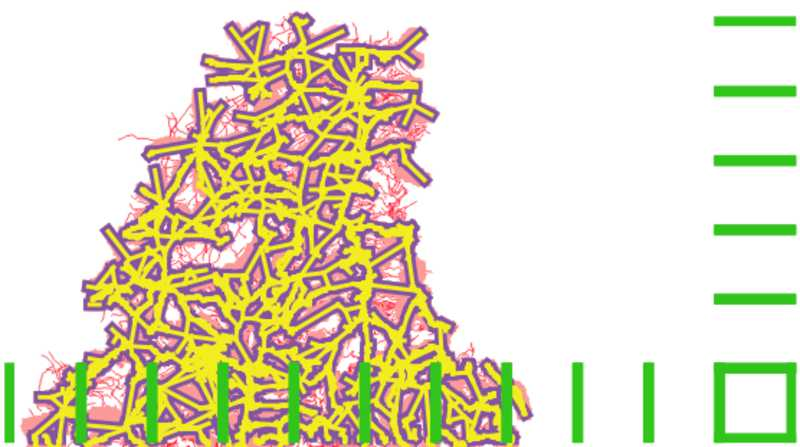
\includegraphics[width=\textheight,angle=90]{Figures/Final/CL-artwork.jpg}
\end{figure}











